\documentclass{revtex4-2}
\usepackage{braket,amsmath,amssymb,graphicx,float,hyperref,paralist}
\numberwithin{equation}{section}
\allowdisplaybreaks
\begin{document}
\title{Multi-channel Kondo model URG}
\author{Abhirup Mukherjee}
\date{\today}
\maketitle
\section{Introduction}
The multi-channel Kondo model is described by the Hamiltonian
\begin{equation}\begin{aligned}
	H = \sum_{k,\alpha,\gamma}\epsilon_{k}^\gamma \hat n^\gamma_{k\alpha} + J\sum_{kk^\prime,\gamma} \vec{S_d}\cdot\vec{s}_{\alpha\alpha^\prime}{c^\gamma_{k\alpha}}^\dagger c^\gamma_{k^\prime\alpha^\prime}~.
\end{aligned}\end{equation}
It is mostly identical to the single-channel Kondo model: \(k,k^\prime\) sum over the momentum states, \(\alpha,\alpha^\prime\) sum over the spin indices and \(\gamma\) sums over the various channels. \(\vec S_d, \vec s\) are the impurity and conduction bath spin vectors. The renormalization at step \(j\) is given by
\begin{equation}\begin{aligned}
	\Delta H_j = \left(c^\dagger T \frac{1}{\hat \omega - H_D}T^\dagger c - T^\dagger c \frac{1}{\hat \omega - H_D}c^\dagger T\right)
\end{aligned}\end{equation}
\begin{equation}\begin{aligned}
	c^\dagger T = J \sum_{k < \Lambda_j, \alpha}\vec{S_d}\cdot\vec{s}_{\beta \alpha}c^\dagger_{q\beta}c_{k\alpha}, &&&H_D = \epsilon_q \tau_{q\beta} + J S_d^z s_q^z
\end{aligned}\end{equation}
Usually we treat the \(\hat \omega\) as number(s) and study the renormalization in the couplings as functions of the quantum fluctuation scales. Each value of the fluctuation scale defines an eigendirection of \(\hat \omega\). We have then essentially traded off the complexity in the non-commutation of the diagonal and off-diagonal terms for all the directions in the manifold of \(\hat \omega\).

Here we will do something different. We will redefine the \(\hat \omega\) by pulling out the off-diagonal term from it: \(\hat \omega \to \hat \omega - H_X\), and then study the renormalization at various orders by expanding the denominator in powers of \(H_X\). Such a redefinition essentially amounts to a rotation of the eigendirections of \(\hat \omega\). This is done in order to extract some information out of \(\hat \omega\), specifically the dependence of the RG equations on the channel number \(K = \sum_\gamma\). This dependence is in principle present even if we do not do such a redefinition and expansion, in the various directions and values of \(\omega\), because those values encode the non-perturbative information regarding scattering at all loops. However, it is difficult to read off this information directly. This step of redefinition followed by expansion is being done with the sole aim of exposing such information. 

The expansion we are talking about is
\begin{equation}\begin{aligned}
	\eta = \frac{1}{\hat \omega - H_D}T^\dagger c = \frac{1}{\omega^\prime - H_D - H_X}T^\dagger c \simeq \frac{1}{\omega^\prime - H_D}T^\dagger c + \frac{1}{\omega^\prime - H_D}H_X \frac{1}{\omega^\prime - H_D} T^\dagger c
\end{aligned}\end{equation}
where \(H_X = J \sum_{k,k^\prime < \Lambda_j, \alpha,\alpha^\prime}\vec{S_d}\cdot\vec{s}_{\alpha \alpha^\prime}c^\dagger_{k\alpha}c_{k^\prime\alpha^\prime}\) is scattering between the entangled electrons.
With this change, the second and third order renormalizations will take the form
\begin{equation}\begin{aligned}
	\Delta H^{(2)}_j = c^\dagger T \frac{1}{\omega^\prime - H_D}T^\dagger c + T^\dagger c \frac{1}{\omega - H_D}c^\dagger T
\end{aligned}\end{equation}
\begin{equation}\begin{aligned}
	\Delta H^{(3)}_j = c^\dagger T \frac{1}{\omega^\prime - H_D} H_X \frac{1}{\omega^\prime - H_D} T^\dagger c + T^\dagger c \frac{1}{\omega - H_D} H_X \frac{1}{\omega - H_D} c^\dagger T
\end{aligned}\end{equation}

\section{Leading order renormalization}
\begin{equation}\begin{aligned}
	\Delta H^{(2)}_j = \underbrace{c^\dagger T \frac{1}{\omega^\prime - H_D}T^\dagger c}_\text{first term}~+~\underbrace{T^\dagger c \frac{1}{\omega - H_D}c^\dagger T}_\text{second term}
\end{aligned}\end{equation}
\subsection{Second term}
\begin{align}
	T^\dagger c \frac{1}{\hat \omega - H_D}c^\dagger T = J^2\sum_{q\beta k k^\prime \alpha \alpha^\prime} c^\dagger_{k^\prime\alpha^\prime} c_{q\beta} \vec{S_d}\cdot\vec{s}_{\alpha^\prime \beta } \frac{1}{\omega - \epsilon_q\tau_{q\beta} - J S_d^z s_q^z}c^\dagger_{q\beta} c_{k\alpha} \vec{S_d}\cdot\vec{s}_{ \beta\alpha}
\end{align}
In the denominator, the state \(q\beta\) is occupied, so we will substitute \(\tau = + \frac{1}{2}\) and \(s_q^z = \beta\). We will also substitute \(\epsilon_q = +D\), because the state was initially unoccupied.
\begin{align}
	T^\dagger c \frac{1}{\hat \omega - H_D}c^\dagger T &= J^2\sum_{q\beta k k^\prime \alpha \alpha^\prime,a,b} c^\dagger_{k^\prime\alpha^\prime} c_{q\beta} S_d^a s^a_{\alpha^\prime \beta} \frac{1}{\omega - \frac{1}{2}D - J \frac{\beta}{2}S_d^z}c^\dagger_{q\beta} c_{k\alpha} S_d^b s^b_{\beta \alpha} \\
	&= J^2\sum_{q\beta k k^\prime \alpha \alpha^\prime,a,b} c^\dagger_{k^\prime\alpha^\prime} c_{q\beta} S_d^a s^a_{\alpha^\prime \beta} \frac{\omega - \frac{1}{2}D + J \frac{\beta}{2}S_d^z }{\left(\omega - \frac{1}{2}D\right)^2 - \frac{1}{16}J^2}c^\dagger_{q\beta} c_{k\alpha} S_d^b s^b_{\beta \alpha} \\
	&= J^2\sum_{q\beta k k^\prime \alpha \alpha^\prime,a,b} c^\dagger_{k^\prime\alpha^\prime} c_{k\alpha} S_d^a s^a_{\alpha^\prime \beta} \frac{\omega - \frac{1}{2}D  +  J S_d^z \frac{\beta}{2}}{\left(\omega - \frac{1}{2}D\right)^2 - \frac{1}{16}J^2} S_d^b s^b_{\beta \alpha} \left(1 - \hat n_{q\beta}\right)
\end{align}
We can perform the sum over the states being decoupled: \(\sum_q \hat n_{q\beta} = \sum_{\epsilon_q = D - |\delta D|}^D = n_j \).
\begin{align}
	T^\dagger c \frac{1}{\hat \omega - H_D}c^\dagger T &= J^2 n_j \sum_{k k^\prime \alpha \alpha^\prime} c^\dagger_{k^\prime\alpha^\prime} c_{k\alpha} \sum_{\beta,a,b}S_d^a s^a_{\alpha^\prime \beta}s^b_{\beta \alpha} \frac{\left(\omega - \frac{1}{2}D\right) + J S_d^z \frac{\beta}{2}}{\left(\omega - \frac{1}{2}D\right)^2 - \frac{1}{16}J^2} S_d^b
\end{align}
We will now simplify the terms individually. The first term, labelled term 3, is simpler:
\begin{equation}\begin{aligned}
	\label{term3_def}
	\text{term 3} = \frac{J^2 n_j \left(\omega - \frac{1}{2}D\right)}{\left(\omega - \frac{1}{2}D\right)^2 - \frac{1}{16}J^2}\sum_{k k^\prime \alpha \alpha^\prime} c^\dagger_{k^\prime\alpha^\prime} c_{k\alpha} \sum_{\beta,a,b}S_d^a S_d^b s^a_{\alpha^\prime \beta}s^b_{\beta \alpha}
\end{aligned}\end{equation}
The final sum can be performed using the following trick. In order to renormalize the Hamiltonian, the two impurity spin operators \(S_d^a\) and \(S_d^b\) have to multiply to produce another spin operator \(S_d^c\) and that will happen only for \(a\neq b\). For \(a \neq b\), we have the relation \(S_d^a S_d^b = \frac{i}{2}\sum_c \epsilon^{abc}S_d^c\).
\begin{equation}\begin{aligned}
	\sum_{a,b,\beta}S_d^a S_d^b s^a_{\alpha^\prime \beta}s^b_{\beta \alpha} = \sum_{a,b}S_d^a S_d^b \left(s^a s^b\right)_{\alpha^\prime \alpha} = -\frac{1}{4}\sum_{a,b,c_1,c_2}\epsilon^{abc_1}\epsilon^{abc_2}S_d^{c_1}\left(s^{c_2}\right)_{\alpha^\prime \alpha} 
\end{aligned}\end{equation}
The double \(\epsilon\) can be evaluated easily: \(\sum_{ab}\epsilon^{abc_1}\epsilon^{abc_2} = \sum_b\left(\delta_{c_1 c_2} - \delta_{b c_2}\delta_{b c_1}\right) = 2 \delta_{c_1 c_2}\). Substituting this gives
\begin{equation}\begin{aligned}
	\label{term1}
	\text{term 3} &= \frac{J^2 n_j \left(\omega - \frac{1}{2}D\right)}{\left(\omega - \frac{1}{2}D\right)^2 - \frac{1}{16}J^2}\sum_{k k^\prime \alpha \alpha^\prime} c^\dagger_{k^\prime\alpha^\prime} c_{k\alpha} \sum_{c} \left(-\frac{1}{2}\right)S_d^c s^c_{\alpha^\prime \alpha} = \left(-\frac{1}{2}\right)\frac{J^2 n_j \left(\omega - \frac{1}{2}D\right)}{\left(\omega - \frac{1}{2}D\right)^2 - \frac{1}{16}J^2}\sum_{k k^\prime \alpha \alpha^\prime} c^\dagger_{k^\prime\alpha^\prime} c_{k\alpha}  \vec{S_d}\cdot\vec{s}_{\alpha^\prime \alpha}
\end{aligned}\end{equation}
The second term takes a bit more work:
\begin{equation}\begin{aligned}
	\text{term 4} = \frac{1}{2}\frac{J^3 n_j }{\left(\omega - \frac{1}{2}D\right)^2 - \frac{1}{16}J^2}\sum_{k k^\prime \alpha \alpha^\prime} c^\dagger_{k^\prime\alpha^\prime} c_{k\alpha} \sum_{\beta,a,b}\beta S_d^a S_d^z  S_d^bs^a_{\alpha^\prime \beta}s^b_{\beta \alpha}
\end{aligned}\end{equation}
Here we will use the identity:
\begin{equation}\begin{aligned}
	\label{identity_SSS}
	S_d^a S_d^z S_d^b = \left(\frac{1}{4}\delta^{az} + \frac{i}{2}\sum_c \epsilon^{azc}S_d^c\right)S_d^b = \left(\frac{1}{4}\delta^{az}S_d^b + \frac{i}{8} \epsilon^{azb}  - \frac{1}{4}\sum_{c_1,c} \epsilon^{azc_1} \epsilon^{c_1 b c} S_d^c\right) = \frac{1}{4}\left(\delta^{az}S_d^b - \delta^{ab}S_d^z + \delta^{bz}S_d^a\right)
\end{aligned}\end{equation}
We have dropped a numerical term because such a term cannot renormalize the Hamiltonian. Substituting this gives
\begin{equation}\begin{aligned}
	\label{term2}
	\text{term 4} &= \frac{J^3 n_j}{\left(\omega - \frac{1}{2}D\right)^2 - \frac{1}{16}J^2} \frac{1}{4}\sum_{k k^\prime \alpha \alpha^\prime,c} c^\dagger_{k^\prime\alpha^\prime} c_{k\alpha} \left(\vec{S_d}\cdot\vec{s}_{\alpha^\prime\alpha} -S_d^z \sum_\beta \beta s^a_{\alpha^\prime\beta} s^a_{\beta\alpha} \right)
\end{aligned}\end{equation}

\subsection{First term}
\begin{align}
	c^\dagger T \frac{1}{\hat \omega - H_D}T^\dagger c = J^2\sum_{q\beta k k^\prime \alpha \alpha^\prime} c^\dagger_{q\beta} c_{k\alpha} \vec{S_d}\cdot\vec{s}_{\beta \alpha} \frac{1}{\omega^\prime - \epsilon_q\tau_{q\beta} - J S_d^z s_q^z}c^\dagger_{k^\prime\alpha^\prime} c_{q\beta} \vec{S_d}\cdot\vec{s}_{\alpha^\prime \beta}
\end{align}
Here the intermediate state is unoccupied, so we put \(\tau = -\frac{1}{2}, s_q^z = -\frac{\beta}{2}\) and since the initial state was occupied, we put \(\epsilon_q = D\).
\begin{align}
	c^\dagger T \frac{1}{\hat \omega - H_D}T^\dagger c &= \sum_{q\beta k k^\prime \alpha \alpha^\prime a b} c^\dagger_{q\beta} c_{k\alpha} S_d^b s^b_{\beta \alpha} \frac{J^2}{\omega^\prime - \frac{1}{2}D + J \frac{\beta}{2}S_d^z }c^\dagger_{k^\prime\alpha^\prime} c_{q\beta} S_d^a s^a_{\alpha^\prime \beta} \\
							   &= J^2\sum_{q\beta k k^\prime \alpha \alpha^\prime a b} c^\dagger_{q\beta} c_{k\alpha} S_d^b s^b_{\beta \alpha} \frac{\left(\omega^\prime - \frac{1}{2}D\right) - J \frac{\beta}{2}S_d^z }{\left(\omega^\prime - \frac{1}{2}D\right)^2 - \frac{1}{16}J^2}c^\dagger_{k^\prime\alpha^\prime} c_{q\beta} S_d^a s^a_{\alpha^\prime \beta}\\
							   &= J^2\sum_{q\beta k k^\prime \alpha \alpha^\prime a b} c^\dagger_{q\beta} c^\dagger_{k^\prime\alpha^\prime}c_{k\alpha} S_d^b s^b_{\beta \alpha} \frac{-\left(\omega^\prime - \frac{1}{2}D\right) + J \frac{\beta}{2}S_d^z}{\left(\omega^\prime - \frac{1}{2}D\right)^2 - \frac{1}{16}J^2} c_{q\beta} S_d^a s^a_{\alpha^\prime \beta} & \left[c_k c^\dagger_{k^\prime} \sim - c^\dagger_{k^\prime}c_k\right] \\
							   &= J^2\sum_{q\beta k k^\prime \alpha \alpha^\prime a b} c^\dagger_{k^\prime\alpha^\prime}c_{k\alpha} S_d^b s^b_{\beta \alpha} \frac{-\left(\omega^\prime - \frac{1}{2}D\right) + J \frac{\beta}{2}S_d^z}{\left(\omega^\prime - \frac{1}{2}D\right)^2 - \frac{1}{16}J^2} S_d^a s^a_{\alpha^\prime \beta} \hat n_{q\beta} \\
							   &= J^2 n_j \sum_{\beta k k^\prime \alpha \alpha^\prime a b} c^\dagger_{k^\prime\alpha^\prime}c_{k\alpha} s^a_{\alpha^\prime \beta}s^b_{\beta \alpha} S_d^b \frac{-\left(\omega^\prime - \frac{1}{2}D\right) + J S_d^z \frac{1}{2}\beta}{\left(\omega^\prime - \frac{1}{2}D\right)^2 - \frac{1}{16}J^2} S_d^a 
\end{align}
We again simplify the terms individually, calling them term 1 and term 2. 
\begin{equation}\begin{aligned}
	\text{term 1} = \frac{-\left(\omega^\prime - \frac{1}{2}D\right)J^2 n_j} {\left(\omega^\prime - \frac{1}{2}D\right)^2 - \frac{1}{16}J^2} \sum_{\beta k k^\prime \alpha \alpha^\prime a b} c^\dagger_{k^\prime\alpha^\prime}c_{k\alpha} s^a_{\alpha^\prime \beta}s^b_{\beta \alpha} S_d^b S_d^a
\end{aligned}\end{equation}
Since this term will renormalize only for \(a \neq b\), we can use \(S_d^b S_d^a = -S_d^a S_d^b\). This gives
\begin{equation}\begin{aligned}
	\text{term 1} = \frac{\left(\omega^\prime - \frac{1}{2}D\right)J^2 n_j} {\left(\omega^\prime - \frac{1}{2}D\right)^2 - \frac{1}{16}J^2} \sum_{\beta k k^\prime \alpha \alpha^\prime a b} c^\dagger_{k^\prime\alpha^\prime}c_{k\alpha} s^a_{\alpha^\prime \beta}s^b_{\beta \alpha} S_d^a S_d^b
\end{aligned}\end{equation}
This is identical to term 3 (eq.~\ref{term3_def}) except for the change \(\omega^\prime \to \omega\). Copying the result from term 3, we get
\begin{equation}\begin{aligned}
	\label{term3}
	\text{term 1} = -\frac{1}{2}\frac{J^2 n_j \left(\omega^\prime - \frac{1}{2}D\right)}{\left(\omega^\prime - \frac{1}{2}D\right)^2 - \frac{1}{16}J^2} \sum_{k k^\prime \alpha \alpha^\prime,c} c^\dagger_{k^\prime\alpha^\prime} c_{k\alpha} \vec{S_d}\cdot\vec{s}_{\alpha^\prime \alpha}
\end{aligned}\end{equation}
The other term is
\begin{equation}\begin{aligned}
	\text{term 2} = \frac{1}{2}\frac{J^3 n_j}{\left(\omega^\prime - \frac{1}{2}D\right)^2 - \frac{1}{16}J^2} \sum_{\beta k k^\prime \alpha \alpha^\prime a b} \beta c^\dagger_{k^\prime\alpha^\prime}c_{k\alpha} s^a_{\alpha^\prime \beta}s^b_{\beta \alpha} S_d^b S_d^z S_d^a 
\end{aligned}\end{equation}
From eq.~\ref{identity_SSS}, we know that \(S_d^b S_d^z S_d^a =  S_d^a S_d^z S_d^b\), which means this term is again identical to its counterpart, term 4.
\begin{equation}\begin{aligned}
	\label{term4}
	\text{term 2} = \frac{J^3 n_j }{\left(\omega^\prime - \frac{1}{2}D\right)^2 - \frac{1}{16}J^2} \frac{1}{4}\sum_{k k^\prime \alpha \alpha^\prime,c} c^\dagger_{k^\prime\alpha^\prime} c_{k\alpha} \left(\vec{S_d}\cdot\vec{s}_{\alpha^\prime\alpha} -S_d^z \sum_{a \beta} \beta s^a_{\alpha^\prime\beta} s^a_{\beta\alpha} \right)
\end{aligned}\end{equation}

\subsection{Total renormalization \(\Delta H^{(2)}\)}
From the formula for the renormalization \(\Delta H^{(2)}\), we write
\begin{equation}\begin{aligned}
	\Delta H^{(2)} = \text{term 1} + \text{term 2} + \text{term 3} + \text{term 4}
\end{aligned}\end{equation}
These four terms are given by eqs.~\ref{term1}, \ref{term2}, \ref{term3} and \ref{term4}. Since the Hamiltonian has particle-hole and \(\mathrm{SU}(2)\) symmetry, we will impose these symmetries by choosing the relation between \(\omega\) and \(\omega^\prime\) such that \(\text{term 2} = \text{term 4}\) and \( \text{term 3} = -\text{term 1}\). The total renormalization at second order is therefore
\begin{equation}\begin{aligned}
	\Delta H^{(2)} = -2 \times \text{term 3} = -\frac{J^2 n_j \left(\omega - \frac{1}{2}D\right)}{\left(\omega - \frac{1}{2}D\right)^2 - \frac{1}{16}J^2} \sum_{k k^\prime \alpha \alpha^\prime,c} c^\dagger_{k^\prime\alpha^\prime} c_{k\alpha} \vec{S_d}\cdot\vec{s}_{\alpha^\prime \alpha}
\end{aligned}\end{equation}
which gives
\begin{equation}\begin{aligned}
	\Delta J^{(2)} = -\frac{J^2 n_j \left(\omega - \frac{1}{2}D\right)}{\left(\omega - \frac{1}{2}D\right)^2 - \frac{1}{16}J^2}
\end{aligned}\end{equation}
For \(\omega < D/2\), we get the flow towards the strong-coupling fixed point. That is, there is an attractive stable fixed point at \(J^* = 4|\omega - D/2|\) for all bare \(J > 0\). We also get a decay towards the local moment fixed point \(J^* = 0\) for \(J < 0\). For \(\omega = -D/2\) and \(J \ll D\), we get the one-loop PMS form. 
\begin{equation}\begin{aligned}
	\Delta J^{(2)} = \frac{J^2 n_j D}{D^2 - \frac{1}{16}J^2} \simeq \frac{J^2 n_j }{D}
\end{aligned}\end{equation}
\section{Next-to-leading order renormalization}
\begin{equation}\begin{aligned}
	\Delta H^{(3)}_j = \underbrace{c^\dagger T \frac{1}{\omega^\prime - H_D} H_X \frac{1}{\omega^\prime - H_D} T^\dagger c}_\text{first term} ~-~ \underbrace{T^\dagger c \frac{1}{\omega - H_D} H_X \frac{1}{\omega - H_D} c^\dagger T}_\text{second term}
\end{aligned}\end{equation}

\subsection{First term}
\begin{equation}\begin{aligned}
	&c^\dagger T \frac{1}{\omega^\prime - H_D} H_X \frac{1}{\omega^\prime - H_D} T^\dagger c\\
	&= \sum_{q, k, k^\prime, k_1,k_2,\atop{\beta, \alpha, \alpha^\prime, \alpha_1,\alpha_2,\atop{l_1,l_2,a,b,c}}} c^\dagger_{q\beta,l_1} c_{k\alpha,l_1} S_d^a s^a_{\beta \alpha} \frac{J^2}{\omega^\prime - \epsilon_q\tau_{q\beta} - J S_d^z s_q^z} S_d^b s^b_{\alpha_1 \alpha_2} c^\dagger_{k_1\alpha_1,l_2}c_{k_2 \alpha_2,l_2} \frac{J}{\omega^\prime - \epsilon_q\tau_{q\beta} - J S_d^z s_q^z} c^\dagger_{k^\prime\alpha^\prime, l_1} c_{q\beta, l_1} S_d^c s^c_{\alpha^\prime \beta}
\end{aligned}\end{equation}
\(q\) sums over the momenta being decoupled. \(k, k^\prime, k_1,k_2\) sum over the momenta not being decoupled. \(\beta, \alpha, \alpha^\prime, \alpha_1,\alpha_2\) sum over the spin indices. \(l_1,l_2\) sum over the channels. We substitute \(s_q^z = -\frac{\beta}{2}\) and \(\epsilon_q \tau_{q\beta} = \frac{D}{2}\). The term inside the summation becomes
\begin{equation}\begin{aligned}
	&J^3 c^\dagger_{q\beta,l_1} c_{k\alpha,l_1} S_d^a s^a_{\beta \alpha} \frac{1}{\omega^\prime - \frac{D}{2} + J \frac{\beta}{2}S_d^z} S_d^b s^b_{\alpha_1 \alpha_2} c^\dagger_{k_1\alpha_1,l_2}c_{k_2 \alpha_2,l_2} \frac{1}{\omega^\prime - \frac{D}{2} + J \frac{\beta}{2}S_d^z} c^\dagger_{k^\prime\alpha^\prime, l_1} c_{q\beta, l_1} S_d^c s^c_{\alpha^\prime \beta}\\
	=&\frac{J^3 c^\dagger_{q\beta,l_1} c_{k\alpha,l_1} S_d^a s^a_{\beta \alpha} \left(\omega^\prime - \frac{D}{2} - J \frac{\beta}{2}S_d^z\right)S_d^b s^b_{\alpha_1 \alpha_2} c^\dagger_{k_1\alpha_1,l_2}c_{k_2 \alpha_2,l_2} \left(\omega^\prime - \frac{D}{2} - J \frac{\beta}{2}S_d^z\right) c^\dagger_{k^\prime\alpha^\prime, l_1} c_{q\beta, l_1} S_d^c s^c_{\alpha^\prime \beta}}{\left[\left(\omega^\prime - \frac{D}{2}\right)^2 - \frac{1}{16}J^2\right]^2} 
\end{aligned}\end{equation}
We will start simplifying this equation by summing over \(q\). \(c^\dagger_{q\beta}\) and \(c_{q\beta}\) can be easily combined to form \(\hat n_{q\beta}\), because they anti-commute with the other momenta. The sum gives \(\sum_q \hat n_{q\beta l_1} = n_j \). This gives (without writing the summations explicitly)
\begin{equation}\begin{aligned}
	\frac{J^3 n_j  c_{k\alpha,l_1} S_d^a s^a_{\beta \alpha} \left(\omega^\prime - \frac{D}{2} - J \frac{\beta}{2}S_d^z\right)S_d^b s^b_{\alpha_1 \alpha_2} c^\dagger_{k_1\alpha_1,l_2}c_{k_2 \alpha_2,l_2} \left(\omega^\prime - \frac{D}{2} - J \frac{\beta}{2}S_d^z\right) c^\dagger_{k^\prime\alpha^\prime, l_1} S_d^c s^c_{\alpha^\prime \beta}}{\left[\left(\omega^\prime - \frac{D}{2}\right)^2 - \frac{1}{16}J^2\right]^2} 
\end{aligned}\end{equation}
The next simplification involves identifying how to contract the operators. The contractions have to be done so as to reproduce the original \(\vec{S_d}\cdot\vec{s}c^\dagger c\) form so that we can read off the renormalization. Currently, there are four distinct electron labels, \(k,k^\prime,k_1,k_2\). There are two ways to contract them. The first is by choosing \(k_1\alpha_1 = k_2\alpha_2\). However, this term vanishes:
\begin{equation}\begin{aligned}
	\sum_{k_1\alpha_1,b}S_d^b s^b_{\alpha_1 \alpha_1} c^\dagger_{k_1\alpha_1,l_2}c_{k_1 \alpha_1,l_2} = \sum_{b,k_1\alpha_1}S_d^b s^b_{\alpha_1 \alpha_1}\hat n_{k_1\alpha_1,l_2} &= \sum_{b}S_d^b \left(\sum_{\alpha_1}s^b_{\alpha_1 \alpha_1}\right) \int_{-D + |\delta D|}^0 d\epsilon \rho(\epsilon)\\
																						      &= \sum_b S_d^b \text{ Trace }(s^b)\int_{-D + |\delta D|}^0 d\epsilon \rho(\epsilon)= 0
\end{aligned}\end{equation}
The other way to contract the indices is by selecting \(k\alpha = k^\prime \alpha^\prime\). Those two operators can again be brought together without any change of sign because there will be an even number of flips. Summing over \(k=k^\prime\) and the channel index \(l_1\) then gives \(\sum_{l_1}\sum_k \left(1 - \hat n_{k\alpha}\right) = \sum_{l_1}\int_{-D + |\delta D|}^ 0 n_j = \frac{1}{2}K n_j N_j\), where \(n_j = \rho |\delta D|\) and \(N_j = \rho D\). \(K = \sum_{l_1}\) is the total number of conduction bath channels. The factor of half is inserted to model the probability of transition appropriately; not all values of \(\epsilon_k\) will contribute equally to the renormalization. The entire expression is now
\begin{equation}\begin{aligned}
	\label{first_term}
	&\sum_{k_1,k_2,\beta,\alpha, \atop{\alpha^\prime, \alpha_1,\alpha_2,\atop{l_2,a,b,c}}}\frac{J^3 K N_j n_j  S_d^a s^a_{\beta \alpha} \left(\omega^\prime - \frac{D}{2} - J \frac{\beta}{2}S_d^z\right)S_d^b s^b_{\alpha_1 \alpha_2} c^\dagger_{k_1\alpha_1,l_2}c_{k_2 \alpha_2,l_2} \left(\omega^\prime - \frac{D}{2} - J \frac{\beta}{2}S_d^z\right) S_d^c s^c_{\alpha^\prime \beta}}{2\left[\left(\omega^\prime - \frac{D}{2}\right)^2 - \frac{1}{16}J^2\right]^2} \\
	&= \frac{J^3 K N_j n_j }{2\left[\left(\omega^\prime - \frac{D}{2}\right)^2 - \frac{1}{16}J^2\right]^2}\sum_{k_1,k_2,\atop{\alpha_1,\alpha_2,l_2}}c^\dagger_{k_1\alpha_1,l_2}c_{k_2 \alpha_2,l_2} \sum_{\beta,\alpha, \atop{a,b,c}}S_d^a s^a_{\beta \alpha} s^b_{\alpha_1 \alpha_2}s^c_{\alpha \beta} \left(\omega^\prime - \frac{D}{2} - J \frac{\beta}{2}S_d^z\right)S_d^b \left(\omega^\prime - \frac{D}{2} - J \frac{\beta}{2}S_d^z\right) S_d^c 
\end{aligned}\end{equation}
We now need to simplify the final summation.
\begin{equation}\begin{aligned}
	\label{final_sum}
\sum_{\beta,\alpha, \atop{a,b,c}}s^a_{\beta \alpha} s^b_{\alpha_1 \alpha_2}s^c_{\alpha \beta} S_d^a \left(\omega^\prime - \frac{D}{2} - J \frac{\beta}{2}S_d^z\right)S_d^b\left(\omega^\prime - \frac{D}{2} - J \frac{\beta}{2}S_d^z\right) S_d^c 
\end{aligned}\end{equation}
The internal product can be evaluated as follows:
\begin{equation}\begin{aligned}
	\label{internal_sum}
	\left(\omega^\prime - \frac{D}{2} - J \frac{\beta}{2}S_d^z\right)S_d^b\left(\omega^\prime - \frac{D}{2} - J \frac{\beta}{2}S_d^z\right) = \left(\omega^\prime - \frac{D}{2}\right)^2 S_d^b - \frac{\beta J}{2}\left(\omega^\prime - \frac{D}{2}\right)\left\{S_d^z, S_d^b\right\} + \frac{J^2}{4}S_d^z S_d^b S_d^z
\end{aligned}\end{equation}
The anticommutator is \(\left\{S_d^z, S_d^b\right\} = \frac{\delta^{bz}}{2}\). The triple operator product is given by eq.~\ref{identity_SSS}: \(S_d^z S_d^b S_d^z = \frac{1}{4}S_d^b\left(2\delta^{bz} - 1\right)\). The right-hand side of eq.~\ref{internal_sum} becomes
\begin{equation}\begin{aligned}
	\left[\left(\omega^\prime - \frac{D}{2}\right)^2 + \frac{J^2}{16} \left(2\delta^{bz} - 1\right)\right]S_d^b - \frac{\beta J}{4}\delta^{bz}\left(\omega^\prime - \frac{D}{2}\right) \equiv \mathcal{C}_1^b S_d^b + \mathcal{C}_2^b
\end{aligned}\end{equation}
Eq.~\ref{final_sum} takes the form
\begin{equation}\begin{aligned}
	\sum_{\beta,\alpha, \atop{a,b,c}}s^a_{\beta \alpha} s^b_{\alpha_1 \alpha_2}s^c_{\alpha \beta}\left(\mathcal{C}_1^b S_d^a S_d^b S_d^c+ \mathcal{C}_2^b S_d^a S_d^c\right)  
\end{aligned}\end{equation}
These spin products can again be evaluated using standard identities:
\begin{equation}\begin{aligned}
	S_d^a S_d^c = \frac{i}{2}\sum_{e}\epsilon^{ace}S_d^e, ~ ~ ~ S_d^a S_d^b S_d^c = \frac{1}{4}\left(\delta^{ab}S_d^c - \delta^{ac}S_d^b + \delta^{bc}S_d^a\right) 
\end{aligned}\end{equation}
We have dropped constant terms in both equations because such terms cannot renormalize the Hamiltonian. This gives, for eq.~\ref{final_sum},
\begin{equation}\begin{aligned}
	\label{Cb1Cb2}
	\sum_{\beta,\alpha, \atop{a,b,c}}s^a_{\beta \alpha} s^b_{\alpha_1 \alpha_2}s^c_{\alpha \beta}\left[\frac{1}{4}\mathcal{C}_1^b \left(\delta^{ab}S_d^c - \delta^{ac}S_d^b + \delta^{bc}S_d^a\right)+ \mathcal{C}_2^b \frac{i}{2}\sum_{e}\epsilon^{ace}S_d^e\right]
\end{aligned}\end{equation}
We take the first term. Define \(\mathcal{C}^b_1 = \mathcal{C}_{11} + \mathcal{C}_{12}\delta^{bz}\). Also note that the indices \(\alpha,\beta\) can be easily summed over: \(\sum_{\alpha\beta}s^a_{\beta\alpha}c^c_{\alpha\beta} = \text{Trace}\left(s^a s^c\right) = \frac{1}{2}\delta^{ac}\). The term in product with \(\mathcal{C}^b_1\) becomes
\begin{equation}\begin{aligned}
	\label{Cb1}
	\frac{1}{2}\sum_{a,b}s^b_{\alpha_1 \alpha_2}\frac{1}{4}\left(\mathcal{C}_{11} + \mathcal{C}_{12}\delta^{bz}\right) \left(2\delta^{ab}S_d^a - S_d^b\right) &= -\frac{1}{8}\sum_{b}s^b_{\alpha_1 \alpha_2}\left(\mathcal{C}_{11} + \mathcal{C}_{12}\delta^{bz}\right)S_d^b = -\frac{1}{8}\left(\mathcal{C}_{11} \vec{S_d}\cdot\vec{s}_{\alpha_1\alpha_2} + \mathcal{C}_{12}s^z_{\alpha_1\alpha_2}S_d^z\right)
\end{aligned}\end{equation}
The term in product with \(\mathcal{C}^b_2\) can be written as
\begin{equation}\begin{aligned}
	- \frac{i J\left(\omega^\prime - \frac{D}{2}\right)}{8}\sum_{\beta,\alpha, \atop{a,b,c}} \delta^{bz}\beta s^a_{\beta \alpha} s^b_{\alpha_1 \alpha_2}s^c_{\alpha \beta}\sum_{e}\epsilon^{ace}S_d^e &= - \frac{i J\left(\omega^\prime - \frac{D}{2}\right)}{8}\sum_{\beta,\alpha, \atop{a,c}} \beta s^a_{\beta \alpha} s^z_{\alpha_1 \alpha_2}s^c_{\alpha \beta}\sum_{e}\epsilon^{ace}S_d^e\\
																									   &=\frac{-iJ\left(\omega^\prime - \frac{D}{2}\right)}{8}\sum_{\beta,a,c,e} \beta \left(s^c s^a\right)_{\beta \beta} s^z_{\alpha_1 \alpha_2}\epsilon^{ace}S_d^e\\
\end{aligned}\end{equation}
Since \(a \neq c\) (\(a=c\) would make \(\epsilon^{ace} = 0\)), we can use \(\left(s^c s^a\right)_{\beta \beta} = \frac{i}{2}\sum_f \epsilon^{caf}s^f_{\beta\beta} = \frac{i\beta}{4}\epsilon^{caz}\). Substituting this gives
\begin{equation}\begin{aligned}
	\label{Cb2}
	\frac{J\left(\omega^\prime - \frac{D}{2}\right)}{32}\sum_{a,c,e} s^z_{\alpha_1 \alpha_2}\epsilon^{ace}\epsilon^{caz}S_d^e = \frac{J\left(\omega^\prime - \frac{D}{2}\right)}{16} s^z_{\alpha_1 \alpha_2}S_d^z
\end{aligned}\end{equation}

Once we note that \(\mathcal{C}_{11} = \left(\omega^\prime - \frac{D}{2}\right)^2 - \frac{1}{16}J^2\) and \(\omega^\prime - D/2 - 2\mathcal{C}_{12}/J = \omega^\prime - D/2 - J/4\) and when we substitute eqs.~\ref{Cb1} and \ref{Cb2} into eq.~\ref{first_term}, we get
\begin{equation}\begin{aligned}
	\label{third_term_1}
	&-\frac{1}{16}\frac{J^3 K N_j n_j }{\left(\omega^\prime - \frac{D}{2}\right)^2 - \frac{1}{16}J^2}\sum_{k_1,k_2,\atop{\alpha_1,\alpha_2,l_2}}c^\dagger_{k_1\alpha_1,l_2}c_{k_2 \alpha_2,l_2} \vec{S_d}\cdot\vec{s}_{\alpha_1\alpha_2} + \frac{J^4 K N_j n_j \left( \omega^\prime - D/2 - J/4 \right) }{32\left[\left(\omega^\prime - \frac{D}{2}\right)^2 - \frac{1}{16}J^2\right]^2}\sum_{k_1,k_2,\atop{\alpha_1,\alpha_2,l_2}} c^\dagger_{k_1 \alpha_1,l_2}c_{k_2 \alpha_2,l_2}S_d^z s^z_{\alpha_1\alpha_2}
\end{aligned}\end{equation}

\subsection{Second term}
\begin{equation}\begin{aligned}
	&T^\dagger c \frac{1}{\omega - H_D} H_X \frac{1}{\omega - H_D} c^\dagger T\\
	&= \sum_{q, k, k^\prime, k_1,k_2,\atop{\beta, \alpha, \alpha^\prime, \alpha_1,\alpha_2,\atop{l_1,l_2,a,b,c}}}c^\dagger_{k^\prime\alpha^\prime, l_1} c_{q\beta, l_1}  S_d^c s^c_{\alpha^\prime \beta} \frac{J^2}{\omega - \epsilon_q\tau_{q\beta} - J S_d^z s_q^z} S_d^b s^b_{\alpha_1 \alpha_2} c^\dagger_{k_1\alpha_1,l_2}c_{k_2 \alpha_2,l_2} \frac{J}{\omega - \epsilon_q\tau_{q\beta} - J S_d^z s_q^z} c^\dagger_{q\beta,l_1} c_{k\alpha,l_1} S_d^a s^a_{\beta \alpha}
\end{aligned}\end{equation}
We take similar steps as before:
\begin{inparaenum}
	\item \(\epsilon_q \tau_{q\beta} = \frac{D}{2}\)
	\item \(s^z_q = \frac{\beta}{2}\)
	\item Sum over \(q\) to get \(n_j\)
	\item Contract \(k\alpha,k^\prime\alpha^\prime\) to get \(K N_j n_j / 2\)
	\item Compute the internal product to obtain \(\mathcal{C}_1^b S_d^b - \mathcal{C}_2^b\)
\end{inparaenum}.
The expression at this point is
\begin{equation}\begin{aligned}
	\label{Cb1Cb2_2}
	\frac{J^3 K N_j n_j }{2\left[\left(\omega - \frac{D}{2}\right)^2 - \frac{1}{16}J^2\right]^2}\sum_{k_1,k_2,\atop{\alpha_1,\alpha_2,l_2}}c^\dagger_{k_1\alpha_1,l_2}c_{k_2 \alpha_2,l_2} \sum_{\beta,\alpha, \atop{a,b,c}}s^a_{\beta \alpha} s^b_{\alpha_1 \alpha_2}s^c_{\alpha \beta} S_d^c \left(\mathcal{C}_1^b S_d^b - \mathcal{C}_2^b\right) S_d^a
\end{aligned}\end{equation}
\(\mathcal{C}^b_1\) is exactly the same as before, the only difference being \(\omega\) replaces \(\omega^\prime\). The sign of \(\mathcal{C}^b_2\) has also flipped, because \(\beta \to -\beta\). The other difference is that \(S_d^a\) and \(S_d^c\) have switched places. Eq.~\ref{Cb1Cb2} is replaced by
\begin{equation}\begin{aligned}
	\label{Cb1Cb2_3}
	\sum_{\beta,\alpha, \atop{a,b,c}}s^a_{\beta \alpha} s^b_{\alpha_1 \alpha_2}s^c_{\alpha \beta}\left[\frac{1}{4}\mathcal{C}_1^b \left(\delta^{ab}S_d^c - \delta^{ac}S_d^b + \delta^{bc}S_d^a\right) + \mathcal{C}_2^b \frac{i}{2}\sum_{e}\epsilon^{ace}S_d^e\right]
\end{aligned}\end{equation}
Note that even though \(\mathcal{C}^b_2\) came with a minus sign in eq.~\ref{Cb1Cb2_2}, that minus sign has been canceled by a second minus sign that arises from the exchange of \(a \leftrightarrow c\) in \(\epsilon^{cae}\). Since eq.~\ref{Cb1Cb2_3} is identical to eq.~\ref{Cb1Cb2}, we can dirctly write down the renormalization in this case:
\begin{equation}\begin{aligned}
	\label{third_term_2}
	-\frac{1}{16}\frac{J^3 K N_j n_j }{\left(\omega - \frac{D}{2}\right)^2 - \frac{1}{16}J^2}\sum_{k_1,k_2,\atop{\alpha_1,\alpha_2,l_2}}c^\dagger_{k_1\alpha_1,l_2}c_{k_2 \alpha_2,l_2} \vec{S_d}\cdot\vec{s}_{\alpha_1\alpha_2} + \frac{J^4 K N_j n_j \left( \omega - D/2 - J/4 \right) }{32\left[\left(\omega - \frac{D}{2}\right)^2 - \frac{1}{16}J^2\right]^2}\sum_{k_1,k_2,\atop{\alpha_1,\alpha_2,l_2}} c^\dagger_{k_1 \alpha_1,l_2}c_{k_2 \alpha_2,l_2}S_d^z s^z_{\alpha_1\alpha_2}
\end{aligned}\end{equation}

\subsection{Total renormalization \(\Delta H^{(3)}\)}
Similar to the one-loop case, we will choose the require \(\omega\) and \(\omega^\prime\) to be related such that the  RG equations are \(\mathrm{Su}(2)\) symmetric; that is, we will require the terms that renormalize only \(S_d^z s^z\) vanish. The total renormalization at this order is obtained by adding eqs.~\ref{third_term_1} and \ref{third_term_2}.
\begin{equation}\begin{aligned}
	\Delta H^{(3)} = -\frac{J^3 K N_j n_j / 8}{\left(\omega - \frac{D}{2}\right)^2 - \frac{1}{16}J^2}\sum_{k_1,k_2,\atop{\alpha_1,\alpha_2,l_2}}c^\dagger_{k_1\alpha_1,l_2}c_{k_2 \alpha_2,l_2} \vec{S_d}\cdot\vec{s}_{\alpha_1\alpha_2}
\end{aligned}\end{equation}
Combining with \(\Delta H^{(2)}\), we get
\begin{equation}\begin{aligned}
	\Delta J = \frac{J^2 n_j \left[2 \left(D - 2\omega\right) - \frac{1}{2}J K N_j\right]}{\left(D - 2\omega\right)^2 - \frac{1}{4}J^2}
\end{aligned}\end{equation}
We choose \(\omega = -D/2\) to get a clearer idea of what the equations say. We also set \(N_j = \rho D\) and \(n_j = \rho |\delta D|\). Quantities with zero in the subscript will denote their values in the bare Hamiltonian. Using \(\delta D = -|\delta D|\), we can write the continuum form of the equation:
\begin{equation}\begin{aligned}
	\frac{\:\mathrm{d}J}{\:\mathrm{d}t} = \frac{J^2 \rho D^2 \left(1 - \frac{1}{8}JK\rho\right)}{D^2 - \frac{1}{16}J^2}
\end{aligned}\end{equation}
where \(dt = \frac{dD}{D}\).

For \(D \gg J\), we can ignore the \(J\) in the denominator, and the equation reduces to the one-loop poor man's scaling form
\begin{equation}\begin{aligned}
	\label{pms_mchannel}
	\frac{\:\mathrm{d}J}{\:\mathrm{d}t} \simeq \frac{J^2 \rho D^2 \left(1 - \frac{1}{8}JK\rho\right)}{D^2} = J^2 \rho \left(1 - \frac{1}{8}JK\rho\right)
\end{aligned}\end{equation}
This equation has a stable fixed point at \(J^* = \frac{8}{\rho K}\).

\begin{figure}[htpb]
	\centering
	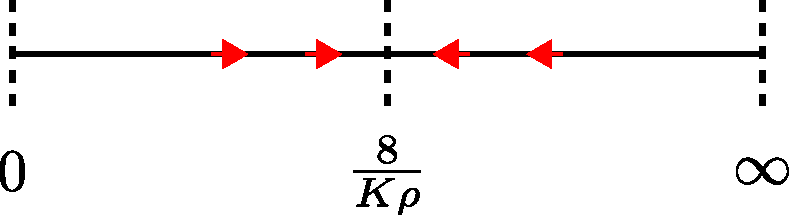
\includegraphics[width=0.4\textwidth]{rg_flow_pms.pdf}
	\caption{Attractive finite \(J\) fixed point of poor man scaling RG equation}
\end{figure}
For \(D\) not so large, the denominator also comes into play, and we get the possibility of two fixed points, one from the numerator and the other from the numerator.
\begin{figure}[htpb]
	\centering
	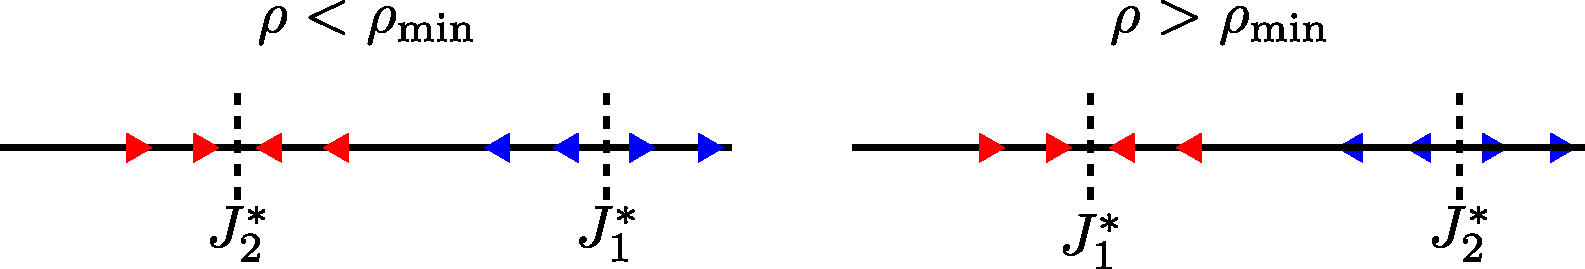
\includegraphics[width=0.7\textwidth]{./rg_flow.pdf}
	\caption{}
	\label{rg_flow_general}
\end{figure}

The numerator fixed point is given by
\begin{equation}\begin{aligned}
	J_1^* = \frac{8}{K \rho}
\end{aligned}\end{equation}
while the denominator fixed point is defined by the condition
\begin{equation}\begin{aligned}
	D^* = \frac{J_2^*}{4}
\end{aligned}\end{equation}
For a given \(K\), the position of \(J_1^*\) will be governed by \(\rho\). In general, for each bare bandwidth \(D_0\), there exists a minimal \(\rho\), $\rho_\text{min}(D_0)$, above which the the lower fixed point is the one from the numerator. That is, for \(\rho > \rho_\text{min}\), if we start scaling from small \(J_0\), it grows until it hits \(J_1^*\) which acts as the attractive fixed point, and \(J_2^*\) lies at a higher value and acts as the repulsive fixed point. For \(\rho < \rho_\text{min}\), \(J\) will grow and hit \(J_2^*\) instead, and \(J_1^* > J_2^*\) now becomes the repulsive fixed point.
\begin{equation}\begin{aligned}
	\rho_\text{min} = \text{minimum }\left\{\rho, \text{ such that } \frac{8}{K \rho} < 4 D^*(\rho)\right\}
\end{aligned}\end{equation}
This behaviour is shown schematically in fig.~\ref{rg_flow_general}. 
In fig.~\ref{rhomin_vs_D}, we plot \(\rho_\text{min}\) against the bare bandwidth. For large \(D_0\), it essentially shrinks to zero, and the numerator becomes the first fixed point for essentially all \(\rho\).
\begin{figure}[htpb]
	\centering
	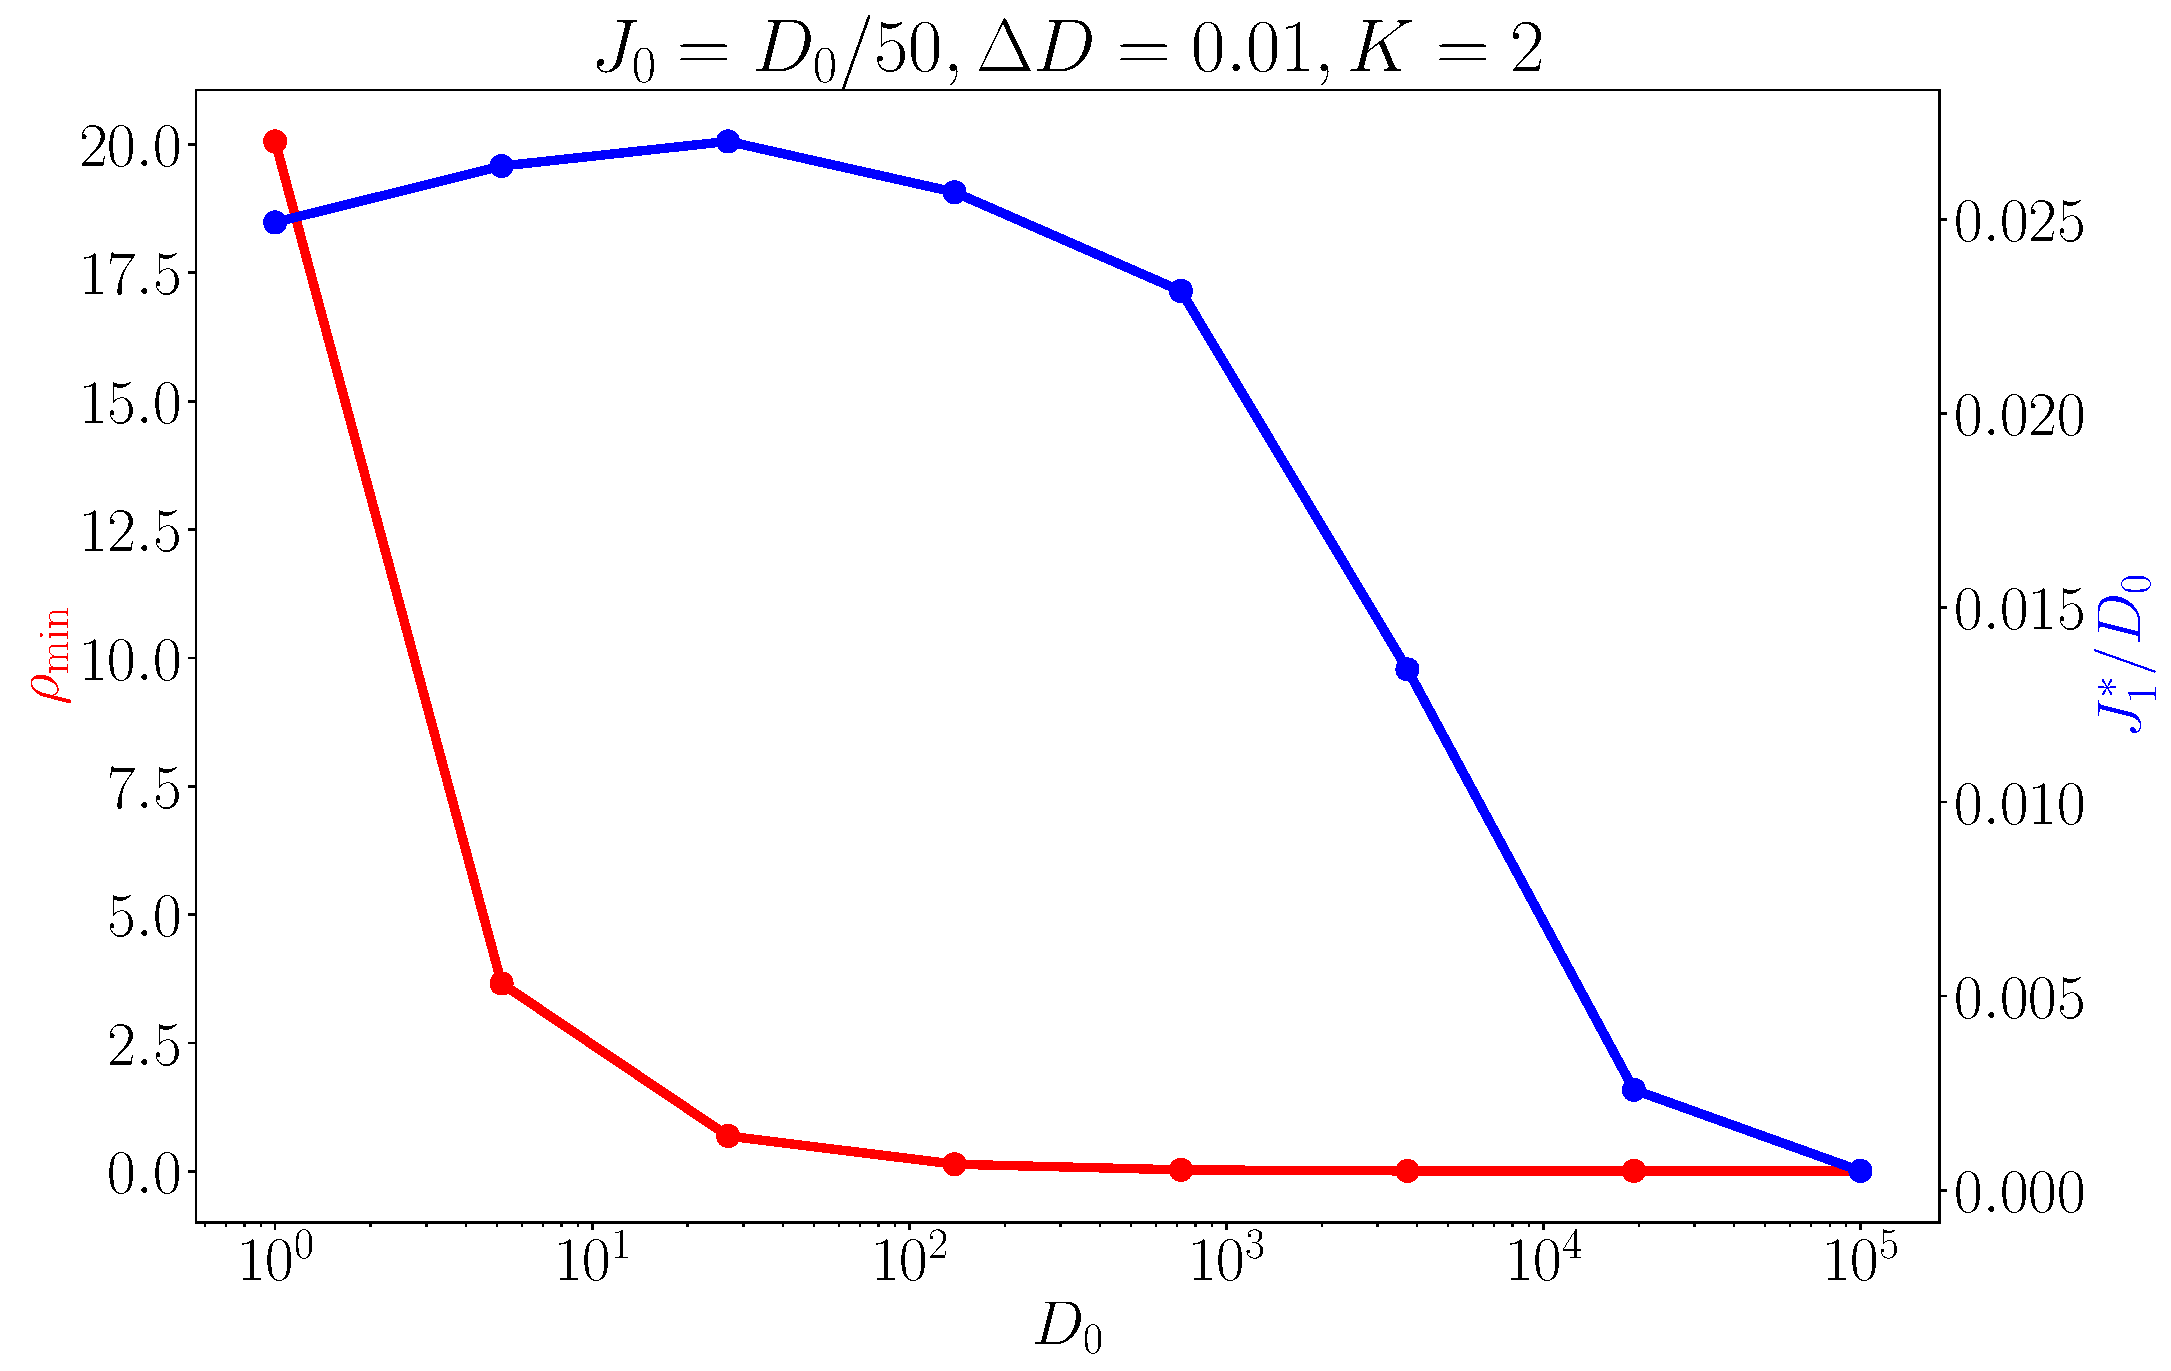
\includegraphics[width=0.7\textwidth]{./rhomin_D.pdf}
	\caption{Red curve shows variation of \(\rho_\text{min}\) against \(D_0\). It vanishes at large \(D_0\). Blue curve shows variation of the ratio \(J_1^* / D_0\) with \(D_0\). That shrinks as well, showing that the fixed point \(J_1^*\) remains finite in the thermodynamic limit, and the distance between \(J_1^*\) and \(J_2^*\) keeps growing.}
	\label{rhomin_vs_D}
\end{figure}

If we assume we are at a sufficiently large \(D_0\) and \(\rho > \rho_\text{min}\), the lower fixed point is \(J_1^*\). As shown in fig.~\ref{rhomin_vs_D}, we have \(J_1^* \ll D_0\). If we start with \(J_0\) in the neighborhood of \(J_1^*\), we can use \(J_1^* \ll D_0\) to ignore \(J\) in the denominator and the RG equation reduces to the poor man's scaling form eq.~\ref{pms_mchannel}. The denominator fixed point has effectively moved off to infinite.

\textbf{\textit{The part of the problem that I have not yet figured out is the following: How do we argue for the same when \(J_0\) is not in the neighborhood of \(J_1^*\)? That is, if \(J_0\) is sufficiently large so that we cannot simpify the denominator. It is true that in order to compete with a thermodynamically large \(D_0\), the bare \(J_0\) will have to be extremely large, and it's possible that this does not even fall in the class of models we are studying.}}

\end{document}
